\documentclass{article}
\usepackage[spanish]{babel}
\usepackage{graphicx}
\usepackage{listings}
\setlength{\parindent}{0pt}
\setlength{\parskip}{3mm}
\usepackage[numbers]{natbib}
\usepackage{color}
\usepackage{booktabs}
\usepackage{subfigure}
%\usepackage{subcaption}
%\usepackage{graphicx,subcaption}
\usepackage{wasysym}

%\usepackage{indentfirst} for APA margins and French indention
\usepackage{url}
%-------------------------------------------------------------------------------
% Configuring customized document margins
%-------------------------------------------------------------------------------
\usepackage{geometry}
%\addtolength{\oddsidemargin}{-.75in}
%\addtolength{\evensidemargin}{-.75in}
%\addtolength{\textwidth}{1.4in}
%
%\addtolength{\topmargin}{-0.25in}
%\addtolength{\textheight}{1.65in}

\definecolor{mygreen}{rgb}{0,0.6,0}
\definecolor{mygray}{rgb}{0.5,0.5,0.5}
\definecolor{mymauve}{rgb}{0.58,0,0.82}
\lstset{ 
  backgroundcolor=\color{white},   % choose the background color; you must add \usepackage{color} or \usepackage{xcolor}; should come as last argument
  basicstyle=\footnotesize,        % the size of the fonts that are used for the code
  breakatwhitespace=false,         % sets if automatic breaks should only happen at whitespace
  breaklines=true,                 % sets automatic line breaking
  captionpos=b,                    % sets the caption-position to bottom
  commentstyle=\color{mygreen},    % comment style
  deletekeywords={...},            % if you want to delete keywords from the given language
  escapeinside={\%}{)},          % if you want to add LaTeX within your code
  extendedchars=true,              % lets you use non-ASCII characters; for 8-bits encodings only, does not work with UTF-8
  firstnumber=1,                % start line enumeration with line 1000
  frame=single,	                   % adds a frame around the code
  keepspaces=true,                 % keeps spaces in text, useful for keeping indentation of code (possibly needs columns=flexible)
  keywordstyle=\color{blue},       % keyword style
  language=Octave,                 % the language of the code
  morekeywords={*,...},            % if you want to add more keywords to the set
  numbers=left,                    % where to put the line-numbers; possible values are (none, left, right)
  numbersep=5pt,                   % how far the line-numbers are from the code
  numberstyle=\tiny\color{mygray}, % the style that is used for the line-numbers
  rulecolor=\color{black},         % if not set, the frame-color may be changed on line-breaks within not-black text (e.g. comments (green here))
  showspaces=false,                % show spaces everywhere adding particular underscores; it overrides 'showstringspaces'
  showstringspaces=false,          % underline spaces within strings only
  showtabs=false,                  % show tabs within strings adding particular underscores
  stepnumber=1,                    % the step between two line-numbers. If it's 1, each line will be numbered
  stringstyle=\color{mymauve},     % string literal style
  tabsize=2,	                   % sets default tabsize to 2 spaces
  title=\lstname                  % show the filename of files included with \lstinputlisting; also try caption instead of title
}



\begin{document}

\title{Tarea No.1: Rectificada}
\author{Dayli Machado de Armas (5275)}
\date{\today}
\maketitle

\section{Gráfo simple no dirigido acíclico}

Un grafo simple no dirigido acíclico, es aquel que no posee dirección en sus aristas, ni bucles, y por supuesto no es reflexivo \cite{Elisa}.

Este tipo de grafos suele representarse por una secuencia de nodos unidos por aristas, donde de cada nodo generalmente solo sale, o llega una arista  \cite{Net}. 

En la práctica este tipo de grafos puede emplearse para representar estructuras moleculares que sigan este comportamiento, por ejemplo, la representación de moléculas. Un ejemplo de estas moléculas sería la representación de alcanos de tipo lineal, donde los átomos serían los nodos y los enlaces entre estos las aristas. Este tipo de moléculas seleccionadas no poseen ciclos, ni bucles en su representación.  Ver figura \ref{fig:Fig01} en la página \pageref{fig:Fig01} donde se muestra la representación gráfica del mismo. 

%\lstinputlisting[language=Python]{Practica.py}
\lstinputlisting[language=Python, firstline=1, lastline=7]{Practica.py}
%\lstinputlisting[language=Python, firstline=9, lastline=58]{codigomadre.py}
\begin{figure}
    \centering
    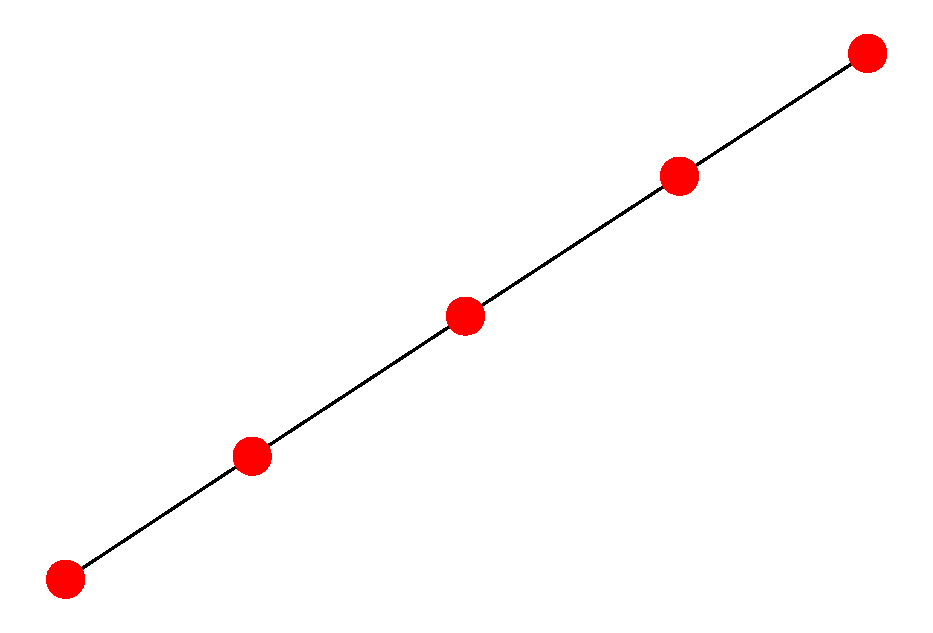
\includegraphics[scale=0.4]{imagenes/Fig01.eps}
    \caption{Representación de grafo simple no dirigido acíclico}
    \label{fig:Fig01}
\end{figure}

\section{Gráfo simple no dirigido cíclico}

Un grafo simple no dirigido cíclico es aquel que no posee dirección en sus aristas, pero si se forma un ciclo que represente una figura cerrada que comience y termine en el mismo vértice, entonces es llamdo cíclico           \cite{redes}. En los grafos no dirigidos, el flujo puede fluir en ambas direcciones.

Este tipo de grafos suele representarse por una secuencia de nodos unidos por aristas, pero estos pueden tener dentro un ciclo, o ser un ciclo en sí mismo. En la práctica, poseen múltiples aplicaciones, por ejemplo en la topología de redes circular, es un ejemplo de aplicación de este tipo de grafo, otro ejemplo pudiera ser la representación de las autopistas de una región dada, o también la representación de otro tipo de moléculas de alcanos, por ejemplo en las de alcanos que se representan como ciclos, siendo el caso del ciclo pentano por ejemplo con cinco nodos unidos por aristas de manera circular. 

El ejemplo a seguir son las llamadas que se realizan interdepartamentales en una muestra de tiempo de la jornada laboral en una empresa determinada, supongamos el departamento de producción, de marketing, comercial, calidad y planificación de la producción, donde cada nodo representa un departamento dentro de la empresa o área de esta, y las aristas las llamadas que se realizan, estas pueden tener un comportamiento que al graficarlo represente un grafo simple no dirigido cíclico. Su utilidad pudiera ser analizar el comportamiento del grafo para minimizar la cantidad de llamadas, o el tiempo de estas por ejemplo.   Ver figura \ref{fig:Fig02} en la página \pageref{fig:Fig02} donde se muestra la representación gráfica del mismo.


\lstinputlisting[language=Python]{grafo2.py}

\begin{figure}
    \centering
    \includegraphics[scale=0.4]{imagenes/Fig02.eps}
    \caption{Representación de grafo simple no dirigido cíclico}
    \label{fig:Fig02}
\end{figure}

\section{Gráfo simple no dirigido reflexivo}

Un grafo simple en el cual  no se permiten aristas multiples, además será no dirigido y reflexivo, si no poseen dirección en sus aristas y reflexivo si cuenta al menos con un bucle, lo que se refiere a una arista reflexiva en la que coinciden el vértice de origen y el vértice de destino \cite{Elisa}. 

Este grafo pudiera emplearse para representar el comportamiento del entrecruzamiento entre diferentes grupos raciales, donde cada grupo representa un nodo diferente, pudiendo existir cruzamiento entre ellos, y las relaciones entre los grupos son los hijos que tengan, es una relación no dirigida, a su vez dentro del grupo de la misma raza se pueden relacionar entre ellos mismos y estarían ocurriendo lazos reflexivos. Si se consideran los cuatro grupos representativos de las razas según la clasificación de especialistas serían: Blanco/caucásico, asiático/mongoloide, negroide/negro y australoide, esta clasificación posee dentro cada grupo una clasificación de hasta 30 subgrupos, pero solo se representarán los cuatro principales. Ver figura \ref{fig:Fig03} en la página \pageref{fig:Fig03} donde se muestra la representación gráfica del mismo.

\lstinputlisting[language=Python]{grafo3.py}

\begin{figure}
    \centering
    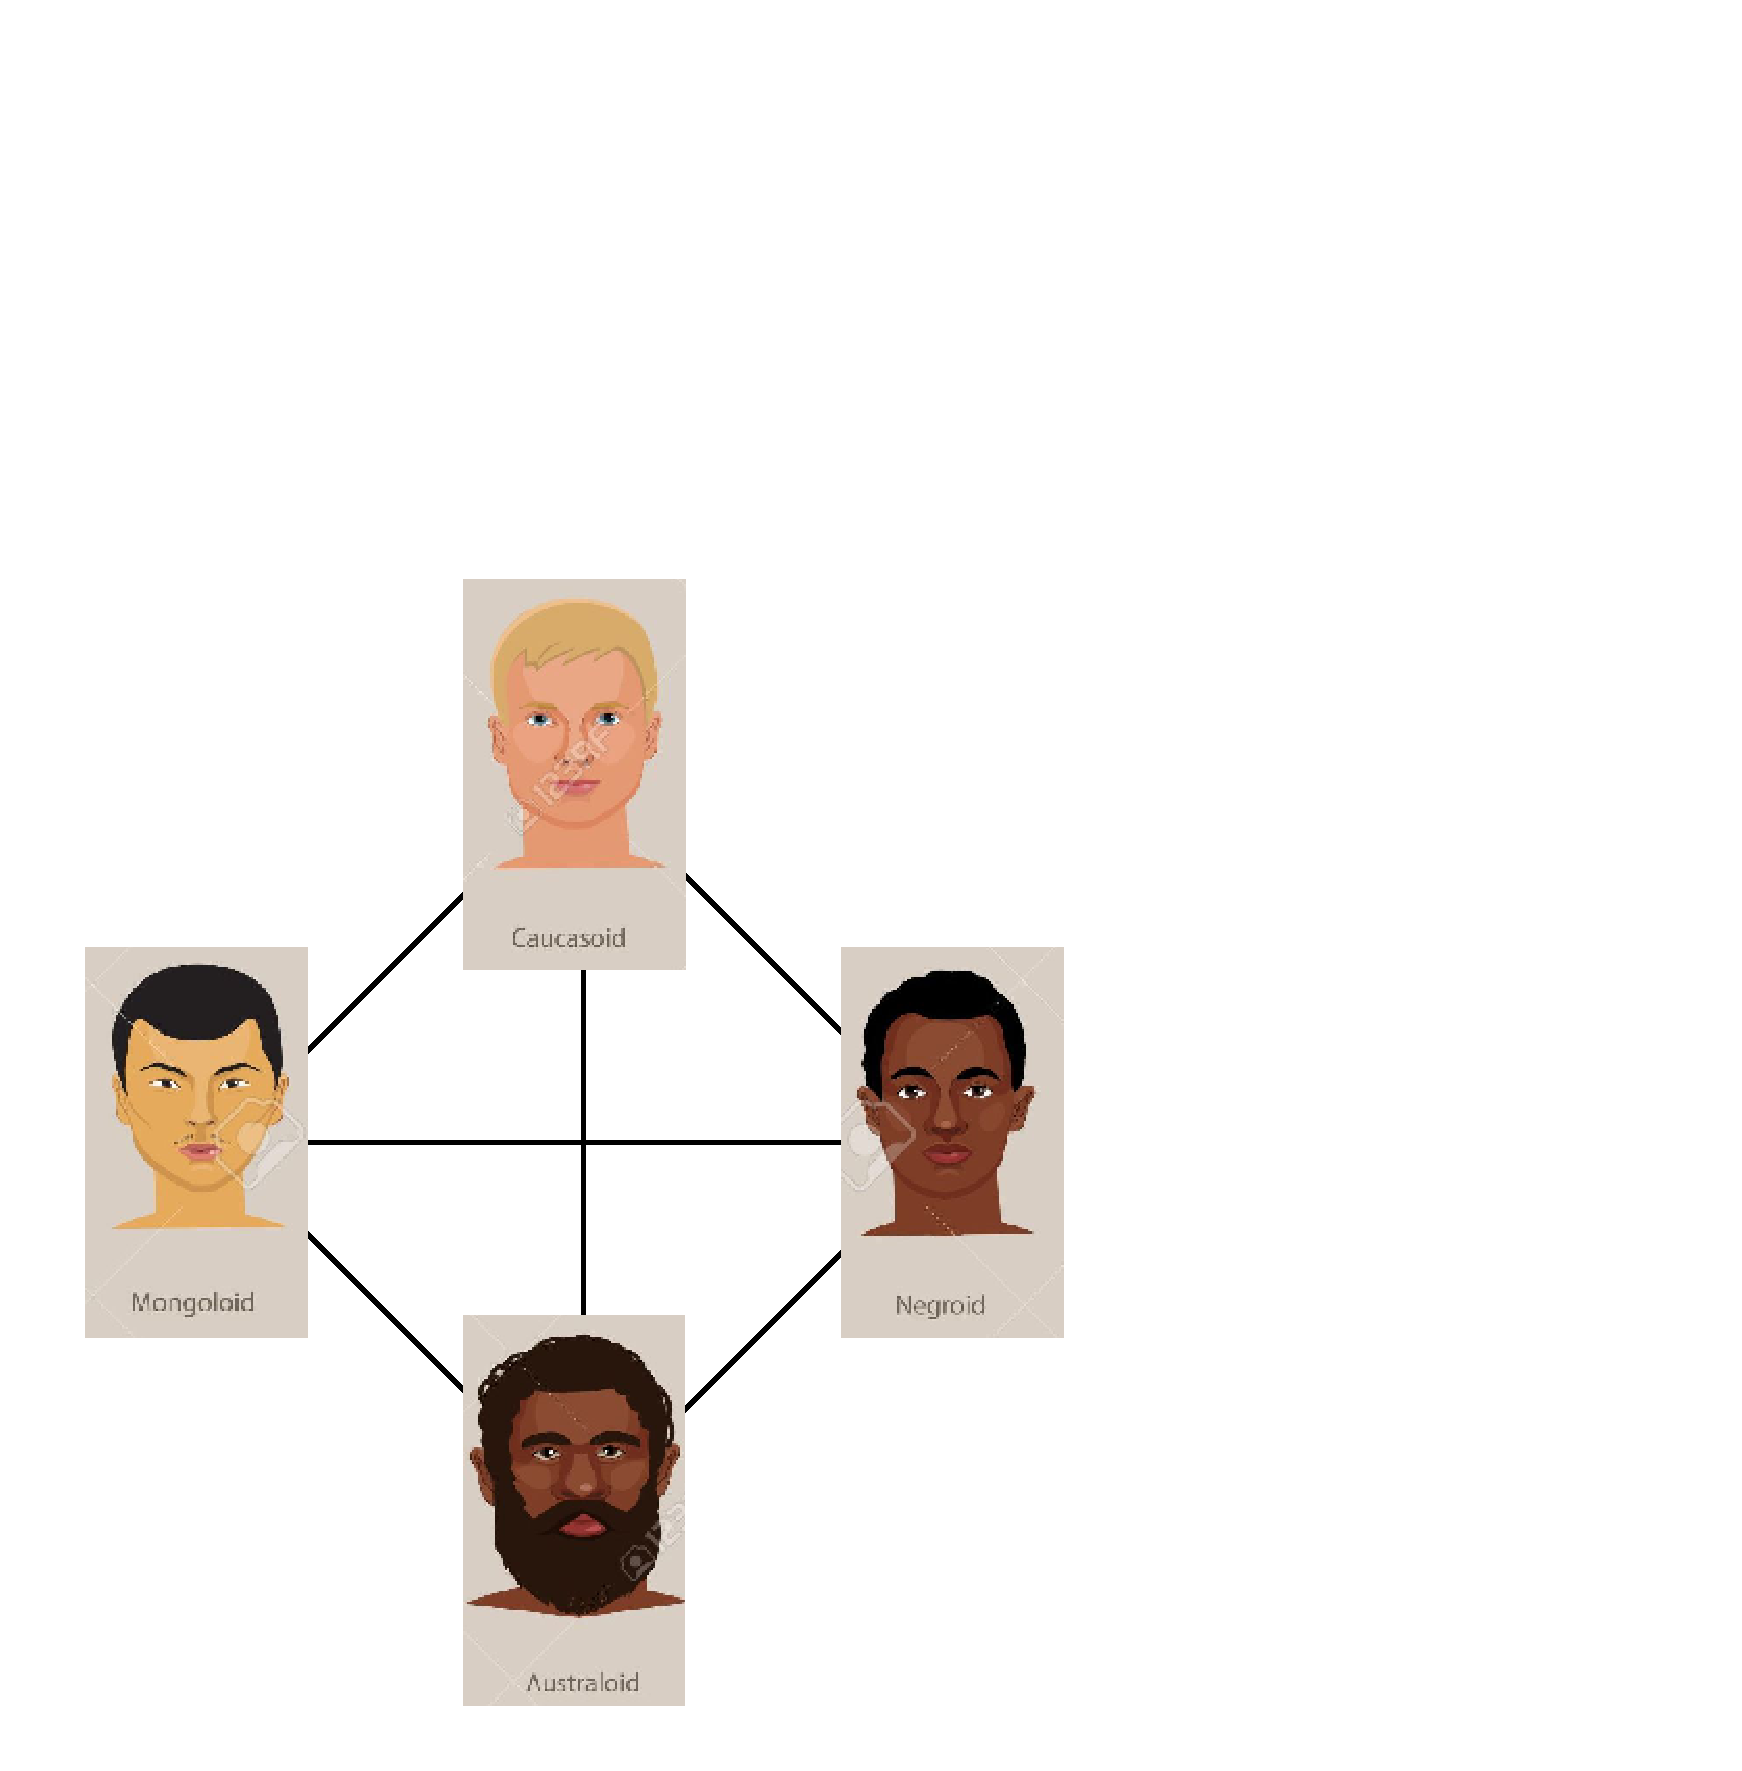
\includegraphics[scale=0.4]{imagenes/Fig03.eps}
    \caption{Representación de grafo simple no dirigido reflexivo}
    \label{fig:Fig03}
\end{figure}

\section{Gráfo simple dirigido acíclico}

Un grafo simple dirigido acíclico, es aquel que posee una dirección en sus aristas, y no posee bucles o reflexividad, ni ciclos\cite{Elisa}.
 
En este caso, ejemplos de la vida real son aquellos que posean un origen del que puede salir una o varias aristas por diferentes caminos, sin que entre ellas existan ciclos y tengan un destino final diferente al del origen. Los árboles genealógicos, los organigramas en las empresas, el flujo de procesos industriales que no posean ciclos, que posean un inicio y un fin, pudieran resultar ser ejemplos de la vida real en los que se puede aplicar este tipo de grafos. Ver figura \ref{fig:Fig04} en la página \pageref{fig:Fig04} donde se muestra la representación gráfica del mismo.


\lstinputlisting[language=Python]{grafo4.py}

\begin{figure}
    \centering
    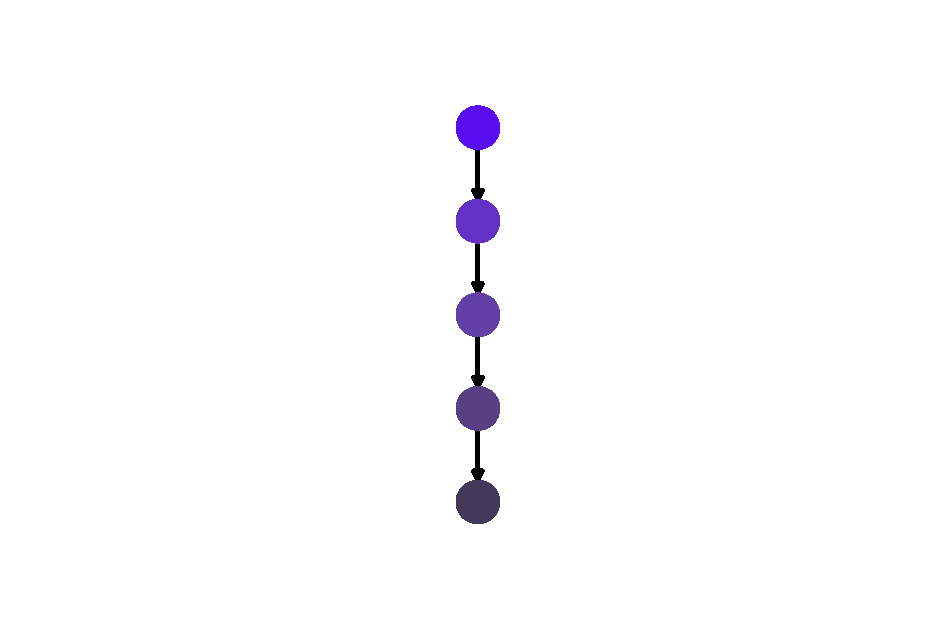
\includegraphics[scale=0.4]{imagenes/Fig04.eps}
    \caption{Representación de gráfo simple dirigido acíclico}
    \label{fig:Fig04}
\end{figure}


\section{Gráfo simple dirigido cíclico}

Un grafo simple dirigido cíclico es aquel que posee una dirección en sus aristas, y posee una figura cerrada que comienza y  termina en el mismo vértice.

En este caso, ejemplos de la vida real son aquellos que posean un origen del que puede salir una o varias aristas por diferentes caminos, y que en un determinado nodo regresen a alguno anterior de modo que se forme uno o más ciclos. El destino final deberá ser diferente al del origen. 

Como aplicación real de este tipo de grafo, puede ser el flujo de procesos industriales o artesanales que posean ciclos, por ejemplo: la elaboración artesanal de jugo de naranja, al representar este proceso en un flujograma mediante un diagrama OPERIN, en el que se reflejen sus operaciones. Una vez que se llegue al paso de exprimir las naranjas que se cae en un ciclo volviendo a la operación anterior de seleccionar otra y otra naranja hasta cubrir toda la capacidad del extractor de jugo. En este ejemplo las operaciones son los nodos  y los enlaces entre los nodos la transformación que va teniendo la naranja durante el proceso. Pudiera representarse como se muestra en la figura \ref{fig:Fig05} en la página \pageref{fig:Fig05} donde se muestra la representación gráfica del mismo.


\lstinputlisting[language=Python]{grafo5.py}

\begin{figure}
    \centering
    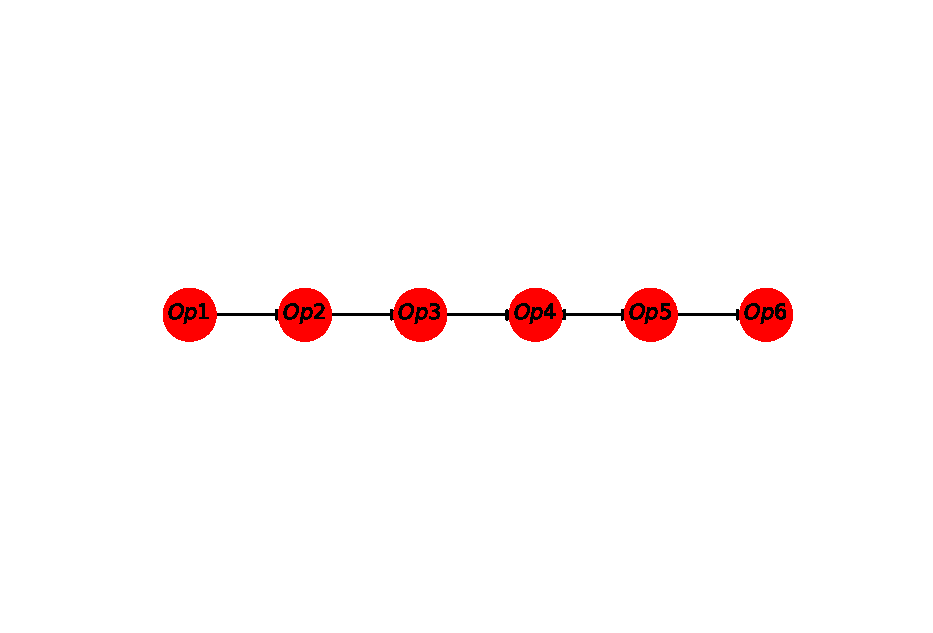
\includegraphics[scale=0.6]{imagenes/Fig05.eps}
    \caption{Representación de gráfo simple dirigido cíclico}
    \label{fig:Fig05}
\end{figure}

\section{Gráfo simple dirigido reflexivo}

La diferencia con este grafo y el anterior reflexivo visto, es que en este caso las aristas si tienen sentido y el flujo que se analice debe ir en una dirección. En este caso deberá existir un nodo que se llame a sí mismo, o sea, que posea al menos un bucle.

Un ejemplo en el que pudiera emplearse la teoría de grafos, y que pudiera seguir un comportamiento dirigido reflexivo es al analizar entre personas de grupos sanguíneos diferentes, representar de quien pueden recibir sangre en función del tipo que posean. La reflexividad está dada en los casos en que cada grupo sanguíneo puede recibir de otros grupos y de sí mismo, excepto el grupo O- que solo puede recibir del mismo tipo.

Pudiera representarse como se muestra en la figura \ref{fig:Fig06} en la página \pageref{fig:Fig06} donde se muestra la representación gráfica del mismo.

\lstinputlisting[language=Python]{grafo6.py}

\begin{figure}
    \centering
    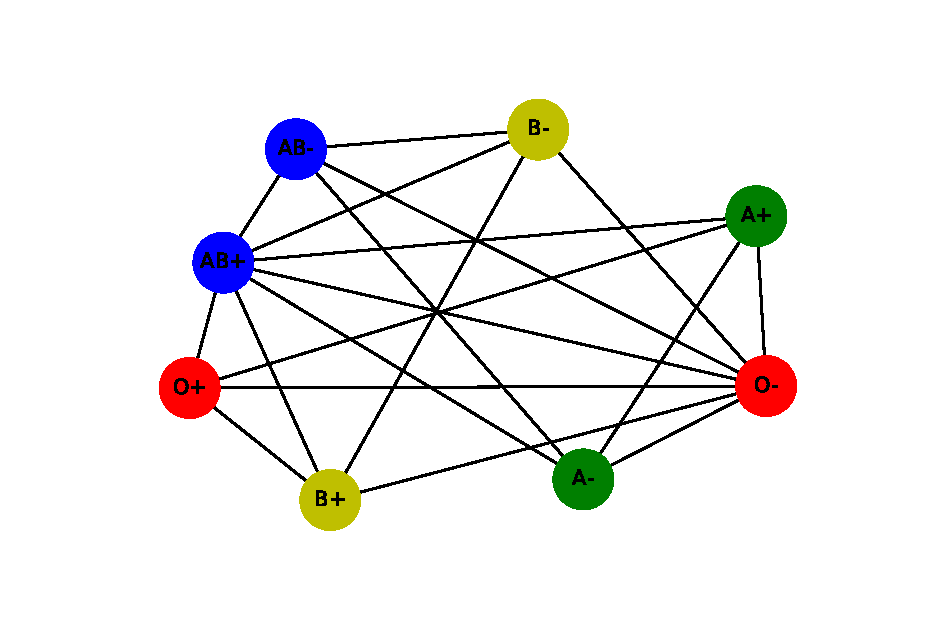
\includegraphics[scale=0.6]{imagenes/Fig06.eps}
    \caption{Representación de gráfo simple dirigido reflexivo}
    \label{fig:Fig06}
\end{figure}

\section{Multigrafo no dirigido acíclico}

Cuando haya más de una arista entre un par de vértices, el grafo se llama multígrafo. Si no se permiten aristas múltiples, el grafo es simple\cite{Elisa}. Es no dirigido cuando las aristas no poseen sentido restringido, sino que el flujo fluye en ambas direcciones, y en este caso no presenta ciclos.

Un ejemplo práctico de multígrafo no dirigido acíclico pudiera decirse que es la representación de determinados enlaces moleculares, como ejemplo pudiera citarse el tipo de elemento que posea un enlace doble éster. Para la representación de los elementos con este tipo de enlace puede emplearse el grafo en cuestión. Específicamente pudiera decirse que la representación de éster sulfúrico pudiera representarse con este comportamiento, como se muestra en la figura \ref{fig:Fig07} en la página \pageref{fig:Fig07} donde se muestra la representación gráfica del mismo. 


\lstinputlisting[language=Python]{grafo7.py}

\begin{figure}
    \centering
    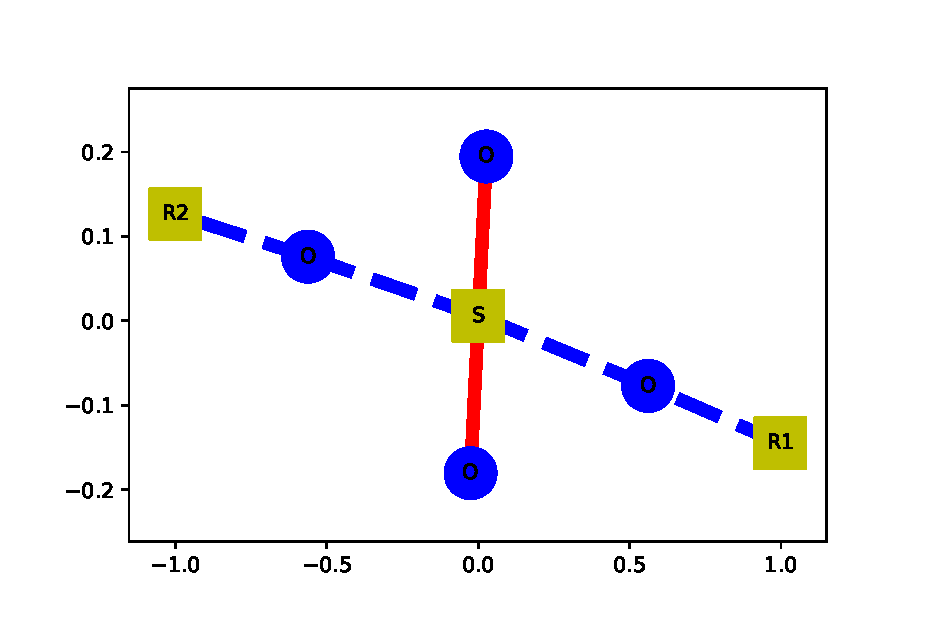
\includegraphics[scale=0.6]{imagenes/Fig07.eps}
    \caption{Representación de multigrafo no dirigido acíclico}
    \label{fig:Fig07}
\end{figure}

\section{Multigrafo no dirigido cíclico}

Cuando haya más de una arista entre un par de vértices, el grafo se llama multígrafo. En este caso será no dirigido cuando las aristas no poseen sentido restringido, sino que el flujo fluye en ambas direcciones, y deberán existir zonas cerradas, o sea, que regresen al nodo inicial.

Este tipo de grafo es de gran utilidad para representar el comportamiento de redes sociales y neuronales por ejemplo. 
El ejemplo práctico que se me ocurre mostrar, es cuando tenemos necesidad de comunicarnos con alguien y las vías de comunicación que tenemos en la actualidad, donde cada vía de comunicación seleccionada tendrá un costo (peso), y existen muchas vías para comunicarnos con otras personas, y a su vez para que esa persona se comunique con nosotros, por lo que no es dirigido, pero sí cíclico, debido a los lazos que se pueden formar entre las personas que necesitan comunicarse. El ejemplo se restringe a solo dos vías de comunicación, ya sea por whatsap, o por llamadas telefónicas, aunque en la práctica existen muchas más. Este grafo se muestra en la figura \ref{fig:Fig08} en la página \pageref{fig:Fig08} donde se muestra la representación gráfica del mismo.

\lstinputlisting[language=Python]{grafo8.py}

\begin{figure}
    \centering
    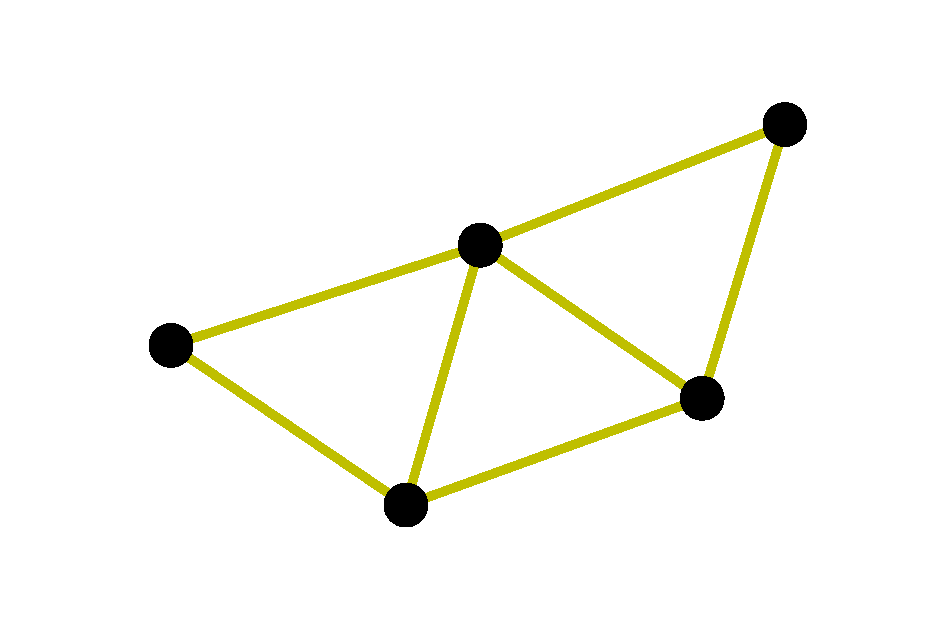
\includegraphics[scale=0.6]{imagenes/Fig08.eps}
    \caption{Representación de Multigrafo no dirigido cíclico}
    \label{fig:Fig08}
\end{figure}

\section{Multigrafo no dirigido reflexivo}

Este caso se refiere a un multigrafo en el existe más de una arista entre un par de vértices, sin dirección entre estas, pero de un nodo deben salir más de una arista que regresen al mismo nodo, sin pasar por otro.

Una aplicación pudiera ser la relación que existe entre cinco signos zodiacales, donde cada nodo representa a las personas de un signo determinado y de cada uno de ellos puede salir una arista que represente las relaciones positivas entre los diferentes signos y otra las relaciones negativas, y a su vez las personas del mismo signo se relacionarán con sus iguales de manera positiva o negativa, lo que representa la reflexibilidad. Este grafo se muestra, para una muestra de cinco signos cualesquiera, en la figura \ref{fig:Fig09} en la página \pageref{fig:Fig09} donde se muestra la representación gráfica del mismo.


\lstinputlisting[language=Python]{grafo9.py}

\begin{figure}
    \centering
    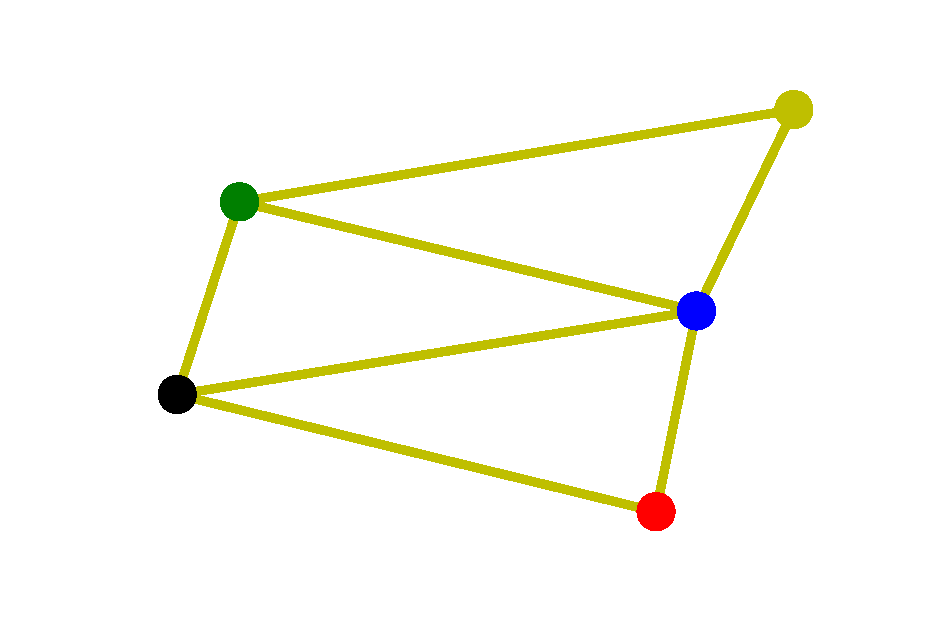
\includegraphics[scale=0.6]{imagenes/Fig09.eps}
    \caption{Representación de Multigrafo no dirigido reflexivo}
    \label{fig:Fig09}
\end{figure}

\section{Multigrafo dirigido acíclico}

Para este tipo de grafo deben existir más de una arista entre un par de nodos, con dirección y no debe formarse ninguna figura cerrada dentro del grafo. 

Este ejemplo aplicado a la práctica pudiera ser la representación de un viajero que desea ir de una ciudad a otra para visitarlas y tiene que elegir entre varias rutas posibles para llegar, o pudiera elegir también entre diferentes medios de transporte para trasladarse entre las ciudades, o una combinación de ambos. En este caso las ciudades serían los nodos, y las rutas o medios de transporte posibles a elegir entre un nodo u otro serían las aristas. Una ruta pudiera ser ir de la ciudad de Matanzas en Cuba, a la Habana, de esta a Monterrey, de Monterrey a Torreón y de ahí a Sinaloa. Este grafo se muestra en la figura \ref{fig:Fig10} en la página \pageref{fig:Fig10} donde se muestra la representación gráfica del mismo. 

\lstinputlisting[language=Python]{grafo10.py}

\begin{figure}
    \centering
    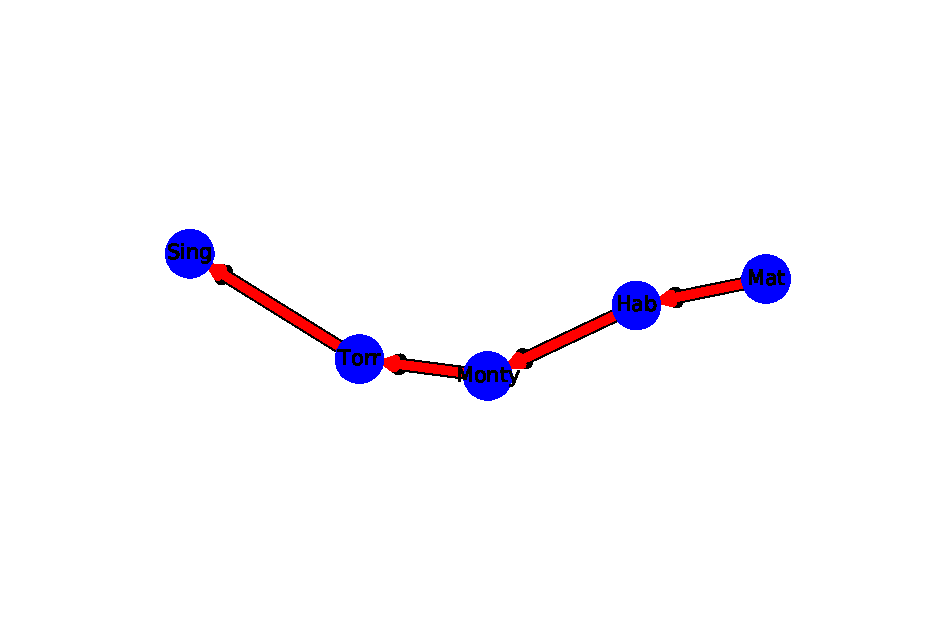
\includegraphics[scale=0.6]{imagenes/Fig10.eps}
    \caption{Representación de multigrafo dirigido acíclico}
    \label{fig:Fig10}
\end{figure}

\section{Multigrafo dirigido cíclico}

Para ser multigrafo dirigido cíclico debe existir más de una arista entre un par de nodos, con dirección y además formarse al menos una figura cerrada dentro del grafo. 

Un ejemplo que representa este tipo de grafo sería la representación del flujo que siguen los pacientes una vez que asisten a la consulta de cuerpo de guardia del ISSSTE, en la que las operaciones del proceso serían los nodos y la clasificación del tipo de paciente y su recorrido dentro de la instalación las aristas. En este caso el cliente al llegar pasa por la consulta de clasificación y ahí le asignan un color en función de la gravedad de su dolencia, se asumen tres colores, rojo, amarillo y verde, que van de mayor gravedad a menor respectivamente y de esta dependerá el tiempo de espera para pasar a la siguiente consulta donde se encuentra el doctor, existe tres consultas con doctores disponibles y de ahí pueden pasar al laboratorio, u a otras de las salas. Luego, del laboratorio pueden pasar nuevamente a la consulta del doctor para revisar los resultados y ocurriría un ciclo, o del doctor directo a la sala, luego al laboratorio y retornar nuevamente al doctor, y ocurriría otro ciclo. Este grafo se muestra en la figura \ref{fig:Fig11} en la página \pageref{fig:Fig11}.

\lstinputlisting[language=Python]{grafo11.py}

\begin{figure}
    \centering
    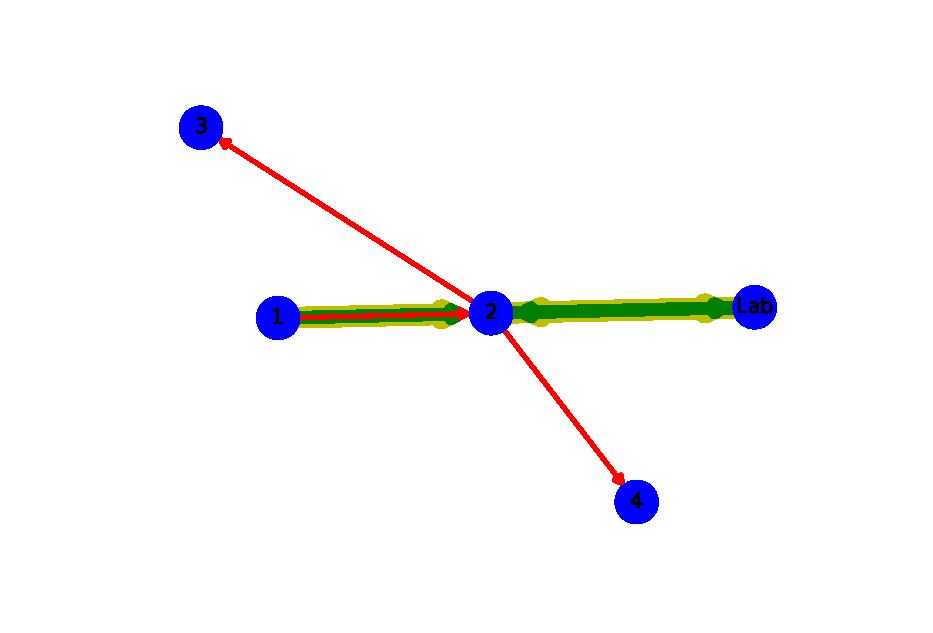
\includegraphics[scale=0.6]{imagenes/Fig11.eps}
    \caption{Representación de multigrafo dirigido cíclico}
    \label{fig:Fig11}
\end{figure}

\section{Multigrafo dirigido reflexivo}

Para ser un multigrafo dirigido reflexivo debe existir más de una arista entre un par de nodos, con dirección y además cada nodo debe llamarse a sí mismo.

Un ejemplo en el que el empleo de la teoría de grafos como los que se analizan en esta sección puede emplearse es en el estudio de la influencia de la religión en la sociedad, como un subejemplo de la aplicación en redes sociales \cite{redes}. 
Por ejemplo, si cada nodo es una persona religiosa creyente, ese nodo (persona) constantemente se realiza un autoexamen de conciencia a sí mismo, evaluando cómo ha sido su actitud con respecto a las variables a analizar en este autoexamen. Estas variables pueden ser operacionalizadas como cada una de las doctrinas de cada religión, las cuales varían de una religión a otra, pero son más de una y pueden agruparse por categorías. Estas variables representan las aristas, cada una puede tener un peso determinado según sea el interés del estudio, a su vez estas mismas doctrinas (convertidas en variable) serán las que cada persona creyente se encargará de transmitir a otras personas creyentes o no, pudiera decirse que se transmite el tipo de actitud que se debe tener ante cada una de estas variables de una persona a otra. 

En este ejemplo se puede evaluar el impacto en un grupo poblacional que puede tener un tipo de creencia u otro, en la medida en que aumente la red. Una simplificación de este tipo de grafo se representa en la figura \ref{fig:Fig12} en la página \pageref{fig:Fig12} donde se muestra la representación gráfica del mismo.

\lstinputlisting[language=Python]{grafo12.py}

\begin{figure}
    \centering
    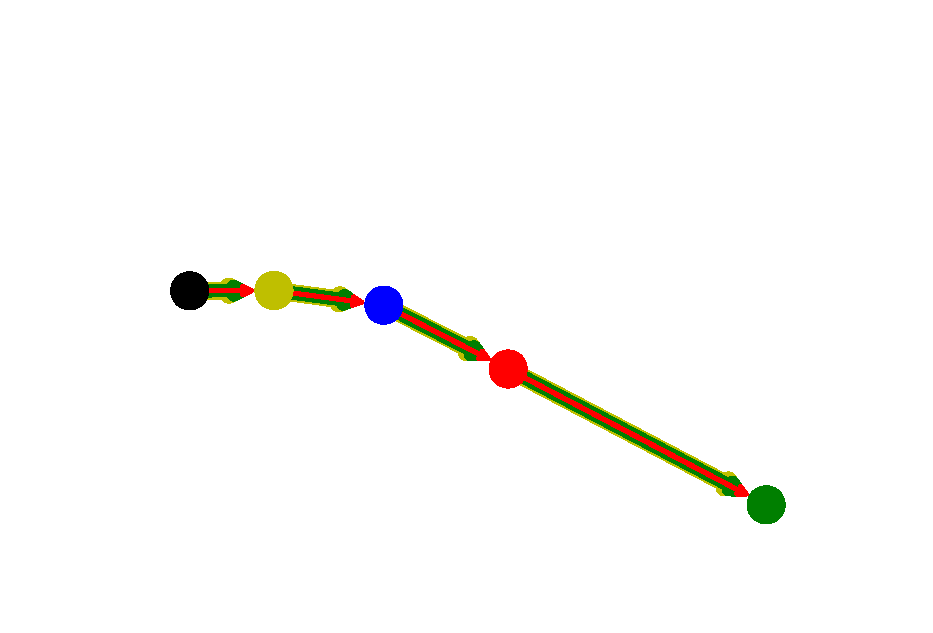
\includegraphics[scale=0.6]{imagenes/Fig12.eps}
    \caption{Representación de multigrafo dirigido reflexivo}
    \label{fig:Fig12}
\end{figure}


\bibliography{Referencias_1}
\bibliographystyle{plainnat}
\end{document}